\documentclass[journal]{IEEEtran}
\usepackage{amsmath,amssymb}
\usepackage{graphicx}
\usepackage{booktabs}
\usepackage{cite}
\usepackage{url}
\usepackage[hidelinks]{hyperref}
% shrink a tabular to the line width only if it is wider than the line
\newsavebox{\fitbox}
\newcommand{\fittab}[1]{\sbox{\fitbox}{#1}\ifdim\wd\fitbox>\linewidth\resizebox{\linewidth}{!}{\usebox{\fitbox}}\else\usebox{\fitbox}\fi}
\newtheorem{proposition}{Proposition}

\begin{document}

\title{AAFV-Net: Reliability-Gated Three-Way Decisions for Adult Cross-Age Face Verification With Audited Random-Impostor False-Accept Risk}

\author{Anurag~Nayak,
        Sujal~Chondhekar,
        Sumit~Kumar,
        Piyush~Jain,
        and~Swati~Hira%
\thanks{The authors are with the Department of Computer Science and Engineering, Indian Institute of Information Technology Nagpur, Nagpur, Maharashtra, India (e-mail: [to be confirmed]; corresponding author: [to be confirmed]).}%
\thanks{Manuscript draft AAFV-06, November 2026. [Funding statement to be confirmed by the authors.]}}

\markboth{AAFV-06 draft (not submitted)}{Nayak \MakeLowercase{\textit{et al.}}: AAFV-Net: Reliability-Gated Three-Way Decisions for Adult Cross-Age Face Verification}

\maketitle

\begin{abstract}
Cross-age face verification must keep impostor admissions rare while the similarity of genuine pairs decays with the time between photographs. AAFV-Net addresses it as a three-way decision---auto-accept, manual review, auto-reject---over a fused score that combines five similarity measures computed on the original pair and on SAM-age-progressed counterparts, gated by image quality, branch-probability floors and a synthesis-reliability score. This paper describes the complete architecture and protocol, reports the logged results on a person-disjoint MORPH test split and on FG-NET, and then audits them. Re-scoring 338,871 MORPH calibration pairs with the frozen model reproduces its published thresholds exactly, which allows controlled, per-pair comparisons. At a matched false-match rate of $10^{-3}$, the fused system ranks pairs no better than ArcFace on the original images; the scores of the generated pairs are weaker than the original-pair scores, and adding them changes the true-accept rate by zero in every gap bin. The previously reported gap in automatic acceptance (70.07\% versus 89.45\% for guarded ArcFace) is produced by the decision layer, and the published operating point exists only because four calibration identities were removed after their scores were inspected; with them restored, the guarded system accepts no genuine pair. The random-impostor false-accept bounds are arithmetically correct but do not distinguish methods. MORPH ``same-person'' pairs with gaps of 15 years or more, as processed, are dominated by linkage errors: 18--29\% record different sexes in their file names and 86--98\% score like random impostors. Image results show that the generator rewrites the periocular region and that the system's external false accepts are infants. We close with a redesigned architecture that uses generated faces only as reliability-weighted training signal, a pre-registered protocol to test it, and the ablations it requires.
\end{abstract}

\begin{IEEEkeywords}
Cross-age face verification, face age progression, three-way decision, reject option, selective verification, false-accept risk, synthetic data, dataset label noise.
\end{IEEEkeywords}

\section{Introduction}
\IEEEPARstart{F}{ace} verification across long time spans is needed when a traveller is compared with an old passport photograph, when an identity credential is renewed after many years, and when a forensic examiner compares a probe with archived images. Aging changes facial texture and soft tissue in adults and facial shape in children, so the similarity of genuine pairs falls as the time between photographs grows~\cite{bestrowden2018longitudinal,deb2018child}, while the impostor distribution does not move. A single decision threshold must then trade false accepts against false rejects, and in high-assurance settings the two errors carry very different costs: an admitted impostor is a security failure, whereas a rejected genuine user can be resolved by a human examiner~\cite{phillips2018pnas}.

Two research directions address the aging problem. Age-invariant recognition changes the representation so that identity is separated from age~\cite{li2011aifr,wang2018oecnn,wang2019dal,huang2021mtlface,zhao2022aim,wang2025ordcon}. Face aging synthesises the missing ages with a generator~\cite{zhang2017caae,tang2018ipcgan,huang2021pfagan,orel2020lifespan,alaluf2021sam,chen2023fading} and uses the synthetic faces as training data~\cite{huang2022mtlfacetpami,banerjee2023aging} or as evidence at verification time. A third, separate literature studies how a deployed classifier should abstain---reject options, selective classification and distribution-free risk control~\cite{chow1970reject,geifman2017selective,angelopoulos2024crc}.

AAFV-Net combines these strands. It treats synthetic age progression as an \emph{auxiliary, unreliable} source of evidence, fuses it with direct similarity under explicit quality and reliability gates, and makes a three-way decision whose accept threshold is set so that no calibration impostor would be accepted (Fig.~\ref{fig:concept}). Earlier versions of this work reported that the system bounded the random-impostor false-accept rate while rejecting most look-alike impostors, together with an unexplained deficit relative to a guarded ArcFace baseline.

This version does three things. First, it documents the complete system---architecture, data, protocol and logged results---in one place (Sections~\ref{sec:method}--\ref{sec:reported}). Second, it audits those results: from recovered models and per-pair feature vectors we reconstruct the frozen pipeline exactly and ask what the generated faces, the fusion network and the decision layer each contribute (Section~\ref{sec:reanalysis}). Third, it uses what the audit shows to propose a redesigned architecture and the protocol needed to test it (Section~\ref{sec:future}). Our contributions are:
\begin{enumerate}
\item A full specification of AAFV-Net, including the corrections found during the audit (the evaluated checkpoint is a three-network ensemble; ArcFace received non-standard alignment).
\item A matched-false-match-rate re-analysis showing that AAFV-Net discriminates no better than ArcFace and that its acceptance deficit is a decision-layer effect.
\item A per-pair test of the generated evidence and a probe of the trained fusion network, showing that the synthetic branch adds no verification evidence on MORPH.
\item An integrity analysis of the calibration procedure and of the false-accept bounds.
\item Evidence, obtainable without images, that MORPH long-gap ``same-person'' pairs in this pipeline are dominated by record-linkage errors, with image results that illustrate it.
\item A redesigned, reliability-weighted age-transport architecture, its ablation plan, and a pre-registered protocol for the question the audit leaves open.
\end{enumerate}

\begin{figure*}[t]
\centering
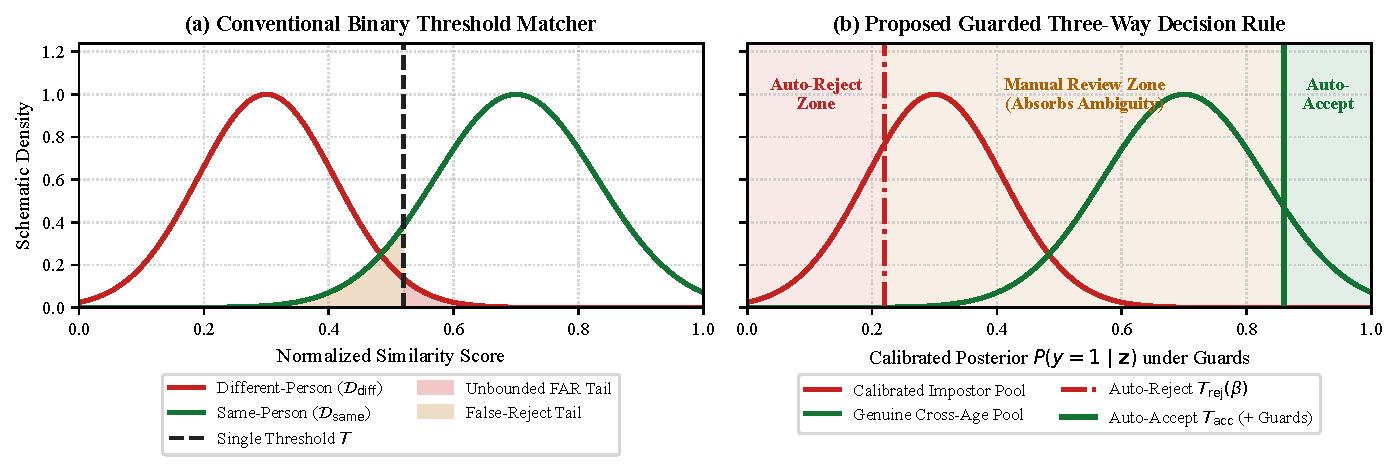
\includegraphics[width=0.88\textwidth]{figures/fig1_concept.pdf}
\caption{Decision concept. (a) A single threshold on a similarity score trades an unbounded false-accept tail against false rejects. (b) AAFV-Net's three-way rule: pairs above $T_\mathrm{acc}$ that pass the guards are auto-accepted, pairs below $T_\mathrm{rej}(\beta)$ are auto-rejected, and the remainder is sent to manual review. Schematic densities.}
\label{fig:concept}
\end{figure*}

\section{Related Work}
\label{sec:related}
\subsection{Age-invariant face recognition}
Early work learned discriminative subspaces for age-invariant matching~\cite{li2011aifr}. Deep methods decompose features into identity and age components (OE-CNN~\cite{wang2018oecnn}), decorrelate them adversarially (DAL~\cite{wang2019dal}), learn them jointly with an aging task (MTLFace~\cite{huang2021mtlface}; AIM~\cite{zhao2022aim}), separate identity and age embeddings with a Wasserstein criterion~\cite{dahan2023wasserstein}, or align feature differences with the ordinal direction of aging (OrdCon~\cite{wang2025ordcon}). These methods retrain the backbone and are evaluated mainly by accuracy on balanced protocols, where strong models now exceed 98\% on AgeDB-30~\cite{moschoglou2017agedb,dahan2023wasserstein}; the informative regime is therefore long gaps at low false-match rates.

\subsection{Face aging and identity preservation}
Conditional generators~\cite{zhang2017caae,tang2018ipcgan,huang2021pfagan}, multi-domain translation~\cite{orel2020lifespan}, StyleGAN latent regression~\cite{karras2020stylegan2,richardson2021psp,alaluf2021sam}, diffusion editing~\cite{chen2023fading,banerjee2023aging}, identity-preserving latent editing~\cite{luevano2025aging} and personalised aging~\cite{qi2025mytimemachine,su2025timebooth} produce increasingly realistic aged faces. Generated faces have been used to fine-tune recognizers after quality-based selection~\cite{huang2022mtlfacetpami,banerjee2023aging}; synthetic identities can also train recognizers from scratch~\cite{boutros2023idiff}. Identity preservation is usually summarised as an average similarity; whether generated faces add evidence at a fixed false-match rate, relative to the recognizer alone, is the question AAFV-Net raises.

\subsection{Recognition backbones, quality and uncertainty}
Margin-based losses (CosFace~\cite{wang2018cosface}, ArcFace~\cite{deng2019arcface}, MagFace~\cite{meng2021magface}, AdaFace~\cite{kim2022adaface}) provide strong generic recognizers; sub-center training tolerates noisy identity labels~\cite{deng2020subcenter}. Face-image quality can be estimated from the recognizer itself~\cite{meng2021magface,terhorst2020serfiq,boutros2023crfiqa}. Probabilistic and data-uncertainty embeddings~\cite{shi2019pfe,chang2020dul,ahn2024ucface} and learned loss attenuation~\cite{kendall2017uncertainty} model per-sample reliability, and verification scores can be calibrated post hoc~\cite{xu2024asc}.

\subsection{Score fusion}
Classical fusion combines matcher scores with fixed rules, density ratios or learned classifiers~\cite{kittler1998combining,ross2003fusion,nandakumar2008lr}; quality-dependent, cost-sensitive fusion with missing channels~\cite{poh2009quality} is the closest precedent for AAFV-Net's reliability-gated synthetic branch.

\subsection{Reject option, risk control and calibration}
Chow derived the optimal error--reject trade-off for known posteriors~\cite{chow1970reject}; learning with rejection~\cite{herbei2006reject} and selective classification~\cite{elyaniv2010selective,geifman2017selective} trade coverage for risk. Conformal prediction and risk control give distribution-free finite-sample guarantees under exchangeability~\cite{vovk2005alrw,angelopoulos2024crc,angelopoulos2021ltt}, with weighted variants under covariate shift~\cite{tibshirani2019covshift}. Scores are mapped to probabilities by Platt scaling, isotonic regression or temperature scaling~\cite{platt1999,zadrozny2002isotonic,guo2017calibration}, and calibration is assessed with ECE and the Brier score~\cite{naeini2015ece,brier1950}.

\subsection{Error estimation, hard impostors, demographics and attacks}
Zero-failure bounds follow from the binomial model~\cite{clopper1934,hanley1983rule3}; comparisons that share subjects require subset or cluster resampling~\cite{bolle2004subsets,schuckers2010book,efron1994bootstrap}, and evaluation practice is standardised in ISO/IEC 19795-1~\cite{iso19795_1}. Look-alikes and twins raise false-match rates~\cite{paone2014twins}, and an adversary can choose impostors strategically~\cite{hu2025neyman}. Accuracy varies with sex, age and race~\cite{klare2012demographics,grother2019frvt_part3,krishnapriya2020race,buolamwini2018gendershades}. Morphing and presentation attacks~\cite{scherhag2019morph,iso30107_3}, template inversion~\cite{otroshi2024inversion} and synthetic-face forgeries~\cite{zhou2024openset} require dedicated defences, and privacy-preserving representations are an active topic~\cite{razeghi2026privacy}.

\section{Problem Formulation and Threat Model}
\label{sec:problem}
A comparison is a pair of aligned face images $(I_1,I_2)$ with ages $a_1\le a_2$, gap $\Delta a=a_2-a_1$ and label $y=1$ for the same person. A scorer produces a probability $P$, two branch probabilities $P_d,P_s$ and a guard indicator $G\in\{0,1\}$. With thresholds $T_\mathrm{rej}<T_\mathrm{acc}$ the decision is
\begin{equation}
\delta=\begin{cases}\text{Accept}, & G=1 \text{ and } P\ge T_\mathrm{acc},\\ \text{Reject}, & P<T_\mathrm{rej},\\ \text{Review}, & \text{otherwise.}\end{cases}
\label{eq:decision}
\end{equation}
For a population of comparisons the false-accept rate is $\mathrm{FAR}=\Pr(\delta=\text{Accept}\mid y=0)$, the false-reject rate $\mathrm{FRR}=\Pr(\delta=\text{Reject}\mid y=1)$ and the genuine coverage $C=\Pr(\delta=\text{Accept}\mid y=1)$. The design objective is to maximise $C$ subject to $\mathrm{FAR}\le\varepsilon$ and $\mathrm{FRR}\le\beta$, with review absorbing the rest.

\begin{proposition}[zero-failure bound]
If $n$ impostor scores $s_1,\dots,s_n$ and a future impostor score are i.i.d.\ given a scorer fixed independently of them, then for any $T\ge\max_i s_i$, $\Pr(\mathrm{FAR}(T)>\varepsilon)\le(1-\varepsilon)^n$, so $\varepsilon=1-\delta^{1/n}$ holds with confidence $1-\delta$; moreover $\mathbb{E}[\mathrm{FAR}(T)]\le 1/(n+1)$~\cite{vovk2005alrw,clopper1934,hanley1983rule3}.
\end{proposition}
This standard argument requires that the scorer, guards and thresholds were not tuned on the $n$ impostors, and that the impostors are exchangeable with future ones. It therefore covers \emph{random}, same-sex adult impostors from the calibration population; mined look-alikes, strategic impostors~\cite{hu2025neyman}, other capture conditions, children, and morphing or presentation attacks~\cite{scherhag2019morph,iso30107_3} are outside its scope and are evaluated empirically or not at all. Section~\ref{sec:integrity} examines whether the conditions hold for AAFV-Net.

\section{AAFV-Net}
\label{sec:method}
Fig.~\ref{fig:arch} shows the system as evaluated. It has five stages.

\begin{figure*}[t]
\centering
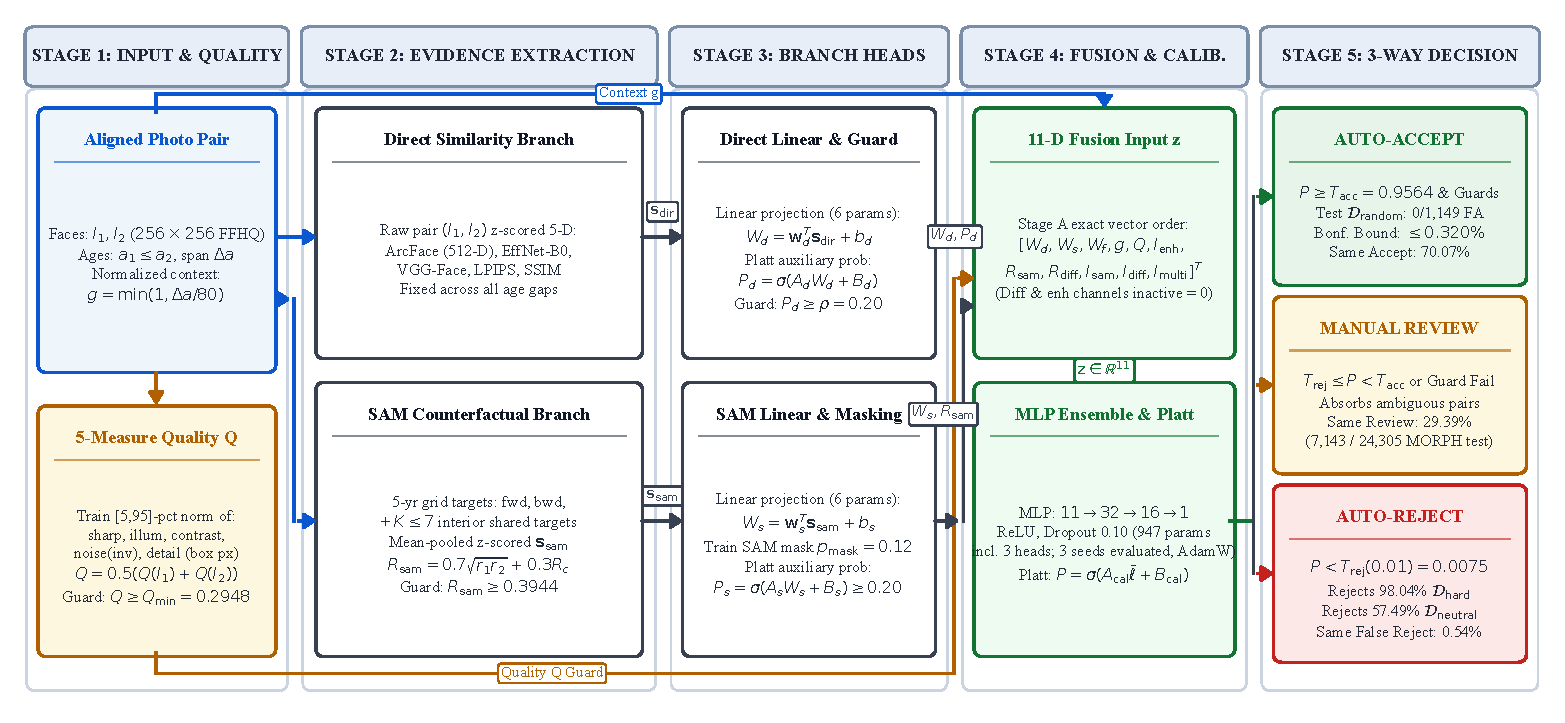
\includegraphics[width=\textwidth]{figures/fig2_architecture.pdf}
\caption{AAFV-Net as evaluated. (1) Alignment and five-measure image quality $Q$. (2) Five similarity measures on the original pair (direct branch) and on SAM-progressed pairs at a 5-year grid of target ages, with synthesis reliability $R_\mathrm{sam}$. (3) One linear head per branch with Platt-scaled branch probabilities; SAM inputs masked during training. (4) An 11-input MLP ensemble and Platt calibration. (5) The guarded three-way rule~\eqref{eq:decision}. Rates are those logged at the second test look (Table~\ref{tab:test}). The ensemble size in the MLP box has been corrected from five to three networks, as found in the frozen checkpoint.}
\label{fig:arch}
\end{figure*}

\subsection{Alignment and image quality}
Faces are detected with dlib~\cite{king2009dlib} (SCRFD~\cite{guo2022scrfd} as fallback) and aligned from 68 landmarks to $256\times256$ FFHQ geometry, the input format of the generator. Image quality combines five measures---Laplacian variance, luminance balance, grey-level contrast, the Immerkær noise estimate~\cite{immerkaer1996noise} (inverted) and detected face-box size---each clipped to its 5th--95th percentile range on the training split and scaled to $[0,1]$:
\begin{equation}
Q(I)=\tfrac{1}{5}\sum_{m=1}^{5}\tilde q_m(I),\qquad Q=\tfrac12\big(Q(I_1)+Q(I_2)\big).
\end{equation}

\subsection{Similarity measures}
For an image pair $(A,B)$ the score vector is $\mathbf s(A,B)=[s_\mathrm{arc},s_\mathrm{eff},s_\mathrm{vgg},d_\mathrm{lpips},s_\mathrm{ssim}]$: cosine similarities of ArcFace~\cite{deng2019arcface}, EfficientNet-B0~\cite{tan2019efficientnet} and VGG-Face~\cite{parkhi2015vgg} descriptors, the LPIPS distance~\cite{zhang2018lpips} and grey-level SSIM~\cite{wang2004ssim}, each z-standardised with training statistics. ArcFace received the $256\times256$ FFHQ crop resized to $112\times112$ rather than its standard five-point alignment; all results below share this choice.

\subsection{Synthetic age-progression evidence}
SAM~\cite{alaluf2021sam} encodes a face into the latent space of StyleGAN2~\cite{karras2020stylegan2} with a pSp encoder~\cite{richardson2021psp} conditioned on a target age. Target ages are snapped to a 5-year grid: the younger image is progressed to $t_\mathrm{fwd}=\mathrm{snap}(a_2)$, the older is regressed to $t_\mathrm{bwd}=\mathrm{snap}(a_1)$, and both are rendered at up to $K_\mathrm{max}=7$ interior grid ages $t_k\in(a_1,a_2)$. With standardised comparison vectors $\mathbf z_\mathrm{fwd},\mathbf z_\mathrm{bwd},\mathbf z_{\mathrm{sh},k}$ and $\mathbf b=\tfrac12(\mathbf z_\mathrm{fwd}+\mathbf z_\mathrm{bwd})$,
\begin{equation}
\mathbf s_\mathrm{sam}=\begin{cases}\tfrac12\mathbf b+\tfrac12\cdot\tfrac{1}{K}\sum_k\mathbf z_{\mathrm{sh},k}, & K\ge1,\\ \mathbf b, & K=0.\end{cases}
\end{equation}

\subsection{Synthesis reliability}
Each generated face receives $r_t=\tfrac13 R_i+\tfrac13 R_a+\tfrac13 Q(\hat I)$, where $R_i=\max(0,\cos(f_\mathrm{arc}(\hat I),f_\mathrm{arc}(I)))$ measures identity agreement with the source, $R_a$ penalises the deviation of the estimated age (DEX~\cite{rothe2018dex}, after removing the pair's estimation bias) from the target, and $Q(\hat I)$ is image quality. Averaging $r_t$ over each face's syntheses gives $r_1,r_2$; with $\sigma_\mathrm{arc}$ the spread of ArcFace cosines across targets,
\begin{equation}
R_\mathrm{sam}=0.7\sqrt{r_1r_2}+0.3\big(1-\min(1,\sigma_\mathrm{arc}/\sigma_\mathrm{max})\big).
\end{equation}
Because $R_i$ uses ArcFace, which is also a fusion input, $R_\mathrm{sam}$ is not an independent identity check.

\subsection{Fusion, masking and calibration}
Linear heads give branch logits $W_d=\mathbf w_d^\top\mathbf s_\mathrm{dir}+b_d$ and $W_s=\mathbf w_s^\top\mathbf s_\mathrm{sam}+b_s$, and separate Platt scalers give $P_d,P_s$. An MLP $11\to32\to16\to1$ (ReLU, dropout 0.1) takes the input
\begin{equation}
\mathbf z=[W_d,W_s,W_f,g,Q,I_\mathrm{enh},R_\mathrm{sam},R_\mathrm{diff},I_\mathrm{sam},I_\mathrm{diff},I_\mathrm{multi}],
\end{equation}
where $g=\min(1,\Delta a/80)$, the $I_\cdot$ are availability flags and four entries are constant placeholders for branches that were not built. Each network has 947 parameters including the three heads; the evaluated checkpoint averages the logits of three networks. Training uses AdamW, batch size 2,048, early stopping on validation log-loss (patience 10), pair weights inverse to gap-bin frequency, and \emph{branch masking}: with probability 0.12 the SAM inputs of a pair are zeroed so the network learns to fall back when synthesis fails. Impostor training pairs number three times the genuine pairs, half random and half the five most ArcFace-similar same-sex images of other persons. The ensemble logit is mapped to $P$ by Platt scaling~\cite{platt1999}, selected over isotonic regression~\cite{zadrozny2002isotonic} by grouped cross-validated log-loss.

\subsection{Guards and thresholds}
A pair may be accepted only if
\begin{multline}
G=\mathbb 1[Q\ge Q_\mathrm{min}]\,\mathbb 1[P_d\ge\rho]\\
\times\big((1-I_\mathrm{sam})+I_\mathrm{sam}\,\mathbb 1[R_\mathrm{sam}\ge R_\mathrm{min}]\,\mathbb 1[P_s\ge\rho]\big)=1,
\end{multline}
with $Q_\mathrm{min}=0.2948$ and $R_\mathrm{min}=0.3944$ (5th percentiles on training data) and $\rho\in\{0.20,0.35,0.50\}$ chosen on calibration data. With $v_{(1)}\ge v_{(2)}\ge\dots$ the sorted $P$ of guard-passing calibration impostors,
\begin{align}
T_\mathrm{acc}&=v_{(1)}+\max\!\big(0.001,\tfrac12(v_{(1)}-v_{(5)})\big),\\
T_\mathrm{rej}(\beta)&=\mathrm{Quantile}_\beta\{P_i: y_i=1\}.
\end{align}
Guards can only move a candidate accept to review; they never cause acceptance or rejection.

\section{Data, Splits and Protocol}
\label{sec:data}
\subsection{Datasets}
MORPH Album~2~\cite{ricanek2006morph} contains longitudinal booking photographs under controlled frontal capture; its subjects are predominantly male and Black or White. An automatic audit found record identifiers that were suffixes of other identifiers or had near-identical embedding centroids; these persons were quarantined. The remaining persons were split person-disjointly into training (with a validation subset), calibration and test partitions. The calibration split contains 338,871 pairs: 23,838 genuine pairs, 1,170 person-disjoint random impostors ($\mathcal{D}_\mathrm{random}$; one image per person, same sex), 278,094 random impostors with repeated persons ($\mathcal{D}_\mathrm{all\,random}$) and 35,769 ArcFace-mined look-alikes ($\mathcal{D}_\mathrm{hard}$). A model-neutral hard set takes the top 1\% of random impostors ranked by independent Siamese models. FG-NET~\cite{lanitis2002fgnet}, with 1,002 scanned images of 82 persons aged 0--69, served as an external set scored with the MORPH-frozen model. Other cross-age datasets---AgeDB~\cite{moschoglou2017agedb}, CACD~\cite{chen2014cacd}, CALFW~\cite{zheng2017calfw}, LAG~\cite{bianco2017lag} and IJB-C~\cite{maze2018ijbc}---were not used and are discussed in Section~\ref{sec:future}.

\subsection{Comparators}
Comparators were scored on the same pairs with the same threshold rule: ArcFace with and without the guards; logistic regression and an MLP on the direct branch only; Siamese networks~\cite{chopra2005siamese} with ResNet-18~\cite{he2016resnet} and ViT-B/16~\cite{dosovitskiy2021vit} backbones (the ViT stopped after three epochs, not converged); and Qwen2-VL-2B~\cite{wang2024qwen2vl} adapted with LoRA~\cite{hu2022lora}, scored on a calibration subset only.

\subsection{Protocol and test budget}
The test split was opened twice under a logged budget (Table~\ref{tab:chronology}). Between the two looks all variants were retrained and the reject rule was changed; Look~2 is therefore a secondary, not a confirmatory, evaluation, and a Bonferroni split of $\delta$ over the two looks controls multiplicity but not adaptivity~\cite{angelopoulos2021ltt}. Rates on correlated pools carry person-clustered bootstrap intervals~\cite{bolle2004subsets,efron1994bootstrap}; binomial bounds are applied only to $\mathcal{D}_\mathrm{random}$.

\begin{table}[t]
\centering
\caption{Protocol chronology reconstructed from logged artifacts and run logs. Steps without a logged time stamp are marked ``not logged''.}
\label{tab:chronology}
\footnotesize
\fittab{\begin{tabular}{@{}p{0.25\linewidth}p{0.68\linewidth}@{}}
\toprule
Time (UTC) & Event \\
\midrule
not logged & Person-level split; automatic quarantine of 854 persons; pair construction; fusion training (5 networks). \\
not logged & Draft calibration: at $\rho=0.20$, $T_\mathrm{acc}=1.0129$ (no acceptance); draft chose $\rho=0.50$, $T_\mathrm{acc}=0.7976$. Contact sheets of the top-scoring impostors reviewed; 4 further persons quarantined; calibration frozen at $\rho=0.20$, $T_\mathrm{acc}=0.956575$. \\
2026-11-05 21:42:09 & Test look 1 (main system; thresholds hash recorded in the log). \\
not logged & All 26 variants re-trained as 3-network ensembles; reject rule changed to the $\beta$-quantile; baselines trained; neutral hard sets defined. \\
2026-11-07 19:45:00 & Test look 2 (8 variants $\times$ 3 values of $\beta$; no hash recorded in the log). \\
after look 2 & FG-NET scored with frozen thresholds; adult cut-off chosen after the child false accepts were seen. \\
\bottomrule
\end{tabular}}
\end{table}


\section{Results as Reported}
\label{sec:reported}
Table~\ref{tab:test} gives the logged results of the second test look. No method accepted a random impostor. AAFV-Net auto-accepted 70.07\% of genuine pairs and auto-rejected 98.04\% of ArcFace-mined look-alikes with five false accepts, whereas guarded ArcFace accepted 89.45\% but rejected none of the look-alikes. The learned end-to-end comparators accepted almost no genuine pairs because their calibration impostor maxima pushed $T_\mathrm{acc}$ to 0.98 or above. Fig.~\ref{fig:outcomes} shows the same pattern on the calibration subset, Table~\ref{tab:ablations} the decision-level ablations, and Table~\ref{tab:fgnet} the FG-NET results: on adults AAFV-Net auto-accepted 51.92\% of genuine pairs against 40.38\% for ArcFace and was higher in every gap bin, but falsely rejected 18.20\% of genuine pairs against a 1\% target; on all ages it made four false accepts in 20,000 impostor pairs, all involving children aged 0--4.

\begin{table*}[t]
\centering
\caption{AAFV-Net and comparators on the person-disjoint MORPH test split as logged at the second test look ($\beta=1\%$). Genuine pairs: 24,305; person-disjoint random impostors $\mathcal{D}_\mathrm{random}$: 1,149; random impostors with repeated persons $\mathcal{D}_\mathrm{all\,random}$: 277,822; ArcFace-mined look-alikes $\mathcal{D}_\mathrm{hard}$: 35,735; model-neutral hard set: 2,790 (not scored for the two Siamese models, which mined it). These are the reported outcomes; Section~\ref{sec:reanalysis} examines what produces them.}
\label{tab:test}
\footnotesize
\fittab{\begin{tabular}{@{}lcccccccc@{}}
\toprule
 & \multicolumn{3}{c}{Genuine pairs (\%)} & \multicolumn{3}{c}{False accepts (count)} & \multicolumn{2}{c}{Auto-reject (\%)} \\
\cmidrule(lr){2-4}\cmidrule(lr){5-7}\cmidrule(l){8-9}
Method & Accept & Review & Reject & $\mathcal{D}_\mathrm{random}$ & $\mathcal{D}_\mathrm{all\,random}$ & $\mathcal{D}_\mathrm{hard}$ & $\mathcal{D}_\mathrm{hard}$ & Neutral \\
\midrule
AAFV-Net (full) & 70.07 & 29.39 & 0.54 & 0 & 0 & 5 & 98.04 & 57.49 \\
AAFV-Net, no shared targets & 83.91 & 15.64 & 0.44 & 0 & 0 & 0 & 97.85 & 53.98 \\
ArcFace, guarded & 89.45 & 9.39 & 1.16 & 0 & 0 & 0 & 0.00 & 28.46 \\
ArcFace, no guards & 93.58 & 5.26 & 1.16 & 0 & 0 & 0 & 0.00 & 28.46 \\
Direct 5-score LogReg & 87.10 & 11.71 & 1.20 & 0 & 0 & 0 & 0.00 & 22.40 \\
Direct-only MLP & 0.00 & 99.50 & 0.50 & 0 & 0 & 0 & 97.77 & 49.96 \\
Siamese ResNet-18 & 0.21 & 99.17 & 0.63 & 0 & 0 & 0 & 9.86 & -- \\
Siamese ViT-B/16 & 0.00 & 99.23 & 0.77 & 0 & 0 & 0 & 10.04 & -- \\
\bottomrule
\end{tabular}}
\end{table*}


\begin{figure*}[t]
\centering
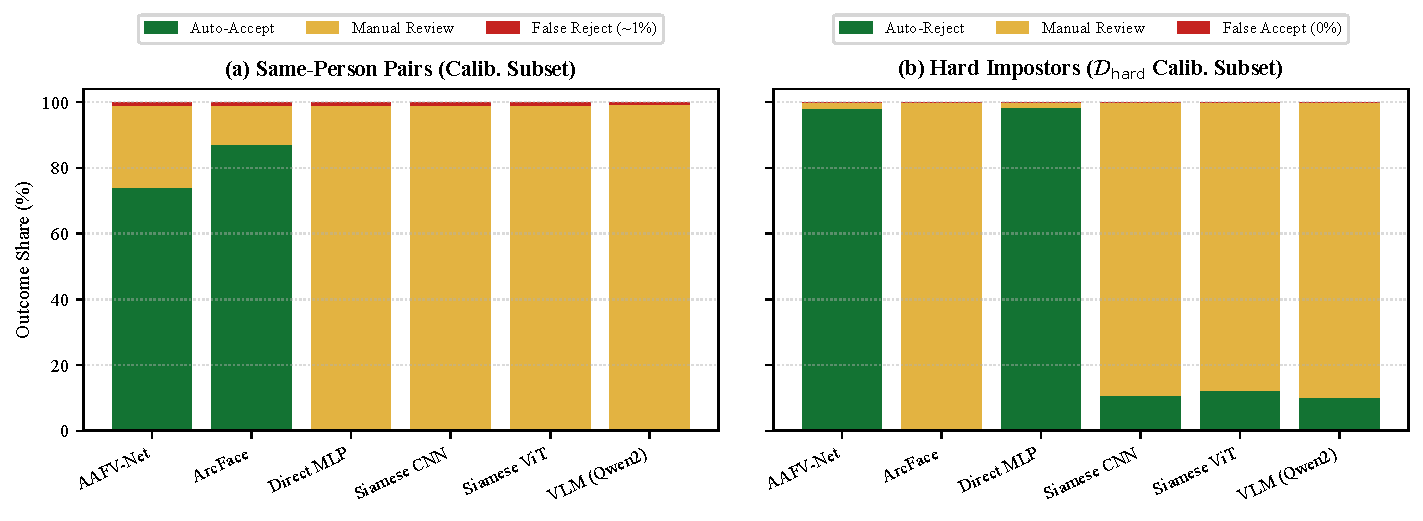
\includegraphics[width=0.9\textwidth]{figures/fig7_decision_outcomes.pdf}
\caption{Three-way outcome shares on the calibration subset for AAFV-Net and comparators. (a) Genuine pairs; (b) ArcFace-mined look-alikes.}
\label{fig:outcomes}
\end{figure*}

\begin{table}[t]
\centering
\caption{Decision-level ablations of AAFV-Net on the calibration common subset (1,500 genuine, 1,170 random and 1,500 mined impostor pairs; $\beta=1\%$), as logged. A threshold above 1 admits nobody; such variants differ in ranking far less than their acceptance suggests (Table~\ref{tab:decision}, Fig.~\ref{fig:gap}).}
\label{tab:ablations}
\footnotesize
\setlength{\tabcolsep}{3pt}
\fittab{\begin{tabular}{@{}lcccc@{}}
\toprule
Variant & $T_\mathrm{acc}$ & Accept (\%) & $\mathcal{D}_\mathrm{hard}$ rej. (\%) & $\mathcal{D}_\mathrm{random}$ rej. (\%) \\
\midrule
\multicolumn{5}{@{}l}{\emph{Full system}} \\
\quad full & 0.956 & 74.13 & 98.20 & 26.15 \\
\multicolumn{5}{@{}l}{\emph{Similarity measures}} \\
\quad drop ArcFace & 0.994 & 0.73 & 17.87 & 52.99 \\
\quad drop EfficientNet & 0.978 & 81.27 & 97.60 & 20.85 \\
\quad drop VGG-Face & 0.976 & 73.93 & 97.20 & 19.57 \\
\quad drop LPIPS & $>1$ & 62.87 & 97.47 & 29.32 \\
\quad drop SSIM & 0.989 & 72.80 & 97.40 & 23.68 \\
\quad ArcFace score only & $>1$ & 0.00 & 97.73 & 24.19 \\
\multicolumn{5}{@{}l}{\emph{Generated evidence}} \\
\quad direct only (no SAM) & $>1$ & 0.00 & 98.47 & 26.67 \\
\quad SAM only & $>1$ & 0.00 & 44.80 & 60.77 \\
\quad no shared targets & 0.997 & 84.80 & 98.27 & 29.23 \\
\quad forward target only & 0.954 & 75.07 & 98.27 & 25.98 \\
\quad shared targets only & $>1$ & 0.00 & 98.13 & 19.06 \\
\quad no $R_\mathrm{sam}$ & 0.989 & 73.27 & 97.80 & 23.85 \\
\quad no branch masking & 0.593 & 3.60 & 98.40 & 30.94 \\
\multicolumn{5}{@{}l}{\emph{Fusion and guards}} \\
\quad logistic fusion (no MLP) & 0.869 & 64.67 & 0.00 & 57.86 \\
\quad no context ($g$, $Q$, $R_\mathrm{sam}$) & $>1$ & 0.00 & 98.07 & 24.70 \\
\quad no pair weights & 0.985 & 74.40 & 97.33 & 24.62 \\
\quad no probability guards & $>1$ & 0.00 & 98.20 & 26.15 \\
\bottomrule
\end{tabular}}
\end{table}

\begin{table*}[t]
\centering
\caption{External evaluation on FG-NET adults (both ages $\geq 16$; cut-off chosen after child false accepts had been observed) with MORPH-frozen models and thresholds. Genuine pairs per gap bin: 405 / 356 / 261 / 170 / 186 / 78. Impostor pairs re-use images of at most 82 persons and are not independent trials. No per-pair scores were logged, so the two methods cannot be compared at a matched false-match rate.}
\label{tab:fgnet}
\footnotesize
\fittab{\begin{tabular}{@{}lccccccccc@{}}
\toprule
 & & & & \multicolumn{6}{c}{Genuine auto-accept by gap (\%)} \\
\cmidrule(l){5-10}
Method & Accept (\%) & False reject (\%) & FA & 0--4 & 5--9 & 10--14 & 15--19 & 20--29 & 30+ \\
\midrule
AAFV-Net & 51.92 & 18.20 & 0/3,670 & 71.6 & 59.6 & 49.0 & 38.2 & 28.5 & 10.3 \\
ArcFace, guarded & 40.38 & 0.27 & 0/3,670 & 60.7 & 49.2 & 35.6 & 25.9 & 14.5 & 3.8 \\
\bottomrule
\end{tabular}}
\end{table*}


Read at face value, these results suggest a trade-off: AAFV-Net automates fewer genuine decisions than ArcFace but filters look-alikes. The rest of the paper tests whether that reading holds.

\section{Re-Analysis}
\label{sec:reanalysis}
\subsection{What was recovered}
The re-analysis uses: the frozen models and decision parameters of all 26 ablation variants, whose SHA-256 hashes match the freeze ledger; the per-pair feature vectors of the calibration split before quarantine (363,647 pairs), from which the official split is recovered exactly by removing the 858 quarantined persons; per-face records for 379,930 SAM-generated and 51,003 original faces; per-variant ranking metrics; logged Look-1 test outputs; and per-pair logits of the Siamese ViT. The test split is not used for any new analysis; logged test outputs are read only descriptively. For a gap bin and impostor pool, the threshold is the smallest impostor score such that the share of impostors above it is at most the target false-match rate (FMR), and TAR is the share of genuine pairs above it. We use FMR $=10^{-3}$, or $10^{-2}$ when a bin holds fewer than 3,000 impostors. Uncertainty comes from a two-way person-cluster bootstrap in which a genuine pair is weighted by its person's multiplicity $c_p$ and an impostor pair by $c_pc_q$; differences between scores are computed on the same replicate (300 replicates).

\subsection{The frozen pipeline is reproduced exactly}
\label{sec:recon}
Re-scoring every calibration pair with the frozen network, calibrator, branch floors and guards reproduces the published accept threshold, reject threshold and genuine acceptance to all reported digits (Table~\ref{tab:reconstruction}, top).

\begin{table}[t]
\centering
\caption{Reconstruction of the frozen decision layer on the MORPH calibration split, and the effect of the four persons removed after the draft calibration. Accept = genuine auto-accept rate. ``None passes'': no impostor passes the guards, which the pipeline encodes as an unattainable threshold.}
\label{tab:reconstruction}
\footnotesize
\fittab{\begin{tabular}{@{}lccc@{}}
\toprule
Quantity (official set, $\rho=0.20$, $n=338,871$ pairs) & Recomputed & Published \\
\midrule
Accept threshold $T_\mathrm{acc}$ & 0.956438 & 0.956438 \\
Reject threshold $T_\mathrm{rej}(\beta{=}0.01)$ & 0.007541 & 0.007541 \\
Genuine auto-accept (\%) & 73.26 & 73.26 \\
\bottomrule
\end{tabular}}

\vspace{4pt}
\fittab{\begin{tabular}{@{}ccccc@{}}
\toprule
 & \multicolumn{2}{c}{Official set} & \multicolumn{2}{c}{Official $+$ 4 persons} \\
\cmidrule(lr){2-3}\cmidrule(l){4-5}
$\rho$ & $T_\mathrm{acc}$ & Accept (\%) & $T_\mathrm{acc}$ & Accept (\%) \\
\midrule
0.20 & 0.9564 & 73.26 & 1.0291 & 0.00 \\
0.35 & 1.0107 & 0.00 & 1.0107 & 0.00 \\
0.50 & none passes & 0.00 & none passes & 0.00 \\
\bottomrule
\end{tabular}}
\end{table}


\subsection{The acceptance deficit is a decision-layer effect}
\label{sec:decision}
Table~\ref{tab:decision} sets each method's auto-accept rate next to threshold-free ranking quality. On the calibration split AAFV-Net auto-accepts 73.3\% of genuine pairs and guarded ArcFace 87.7\%, yet their TAR at FMR $10^{-3}$ against random impostors is 0.977 and 0.980, and their AUCs differ in the third decimal. Per gap bin (Fig.~\ref{fig:gap}) the two are indistinguishable in TAR wherever data exist. The difference in automation arises because each method's zero-calibration-false-accept threshold falls at a different place and because AAFV-Net's guards demote further pairs to review. The guard variants have identical ranking metrics, confirming that guards act only on the threshold.

\begin{table}[t]
\centering
\caption{Decision rate versus ranking quality on the MORPH calibration split. The auto-accept rate depends on where each method's zero-false-accept threshold falls; the threshold-free ranking metrics show that the methods discriminate almost identically. A threshold $\geq 1$ (``none'') admits nobody.}
\label{tab:decision}
\footnotesize
\setlength{\tabcolsep}{3pt}
\fittab{\begin{tabular}{@{}lcccccc@{}}
\toprule
 & & & \multicolumn{2}{c}{Random impostors} & \multicolumn{2}{c}{ArcFace-mined} \\
\cmidrule(lr){4-5}\cmidrule(l){6-7}
Method & $T_\mathrm{acc}$ & Accept (\%) & TPR@$10^{-3}$ & AUC & TPR@$10^{-3}$ & AUC \\
\midrule
AAFV-Net (full) & 0.956 & 73.3 & 0.977 & 0.987 & 0.973 & 0.998 \\
ArcFace, guarded & 0.850 & 87.7 & 0.980 & 0.992 & 0.969 & 0.980 \\
ArcFace, no guards & 0.850 & 92.0 & 0.980 & 0.992 & 0.969 & 0.980 \\
Direct 5-score LogReg & 0.913 & 84.9 & 0.981 & 0.992 & 0.971 & 0.981 \\
Direct-only MLP (no SAM) & none & 0.0 & 0.977 & 0.987 & 0.971 & 0.998 \\
AAFV-Net, no shared targets & 0.997 & 83.6 & 0.977 & 0.987 & 0.974 & 0.998 \\
\bottomrule
\end{tabular}}
\end{table}


\begin{figure}[t]
\centering
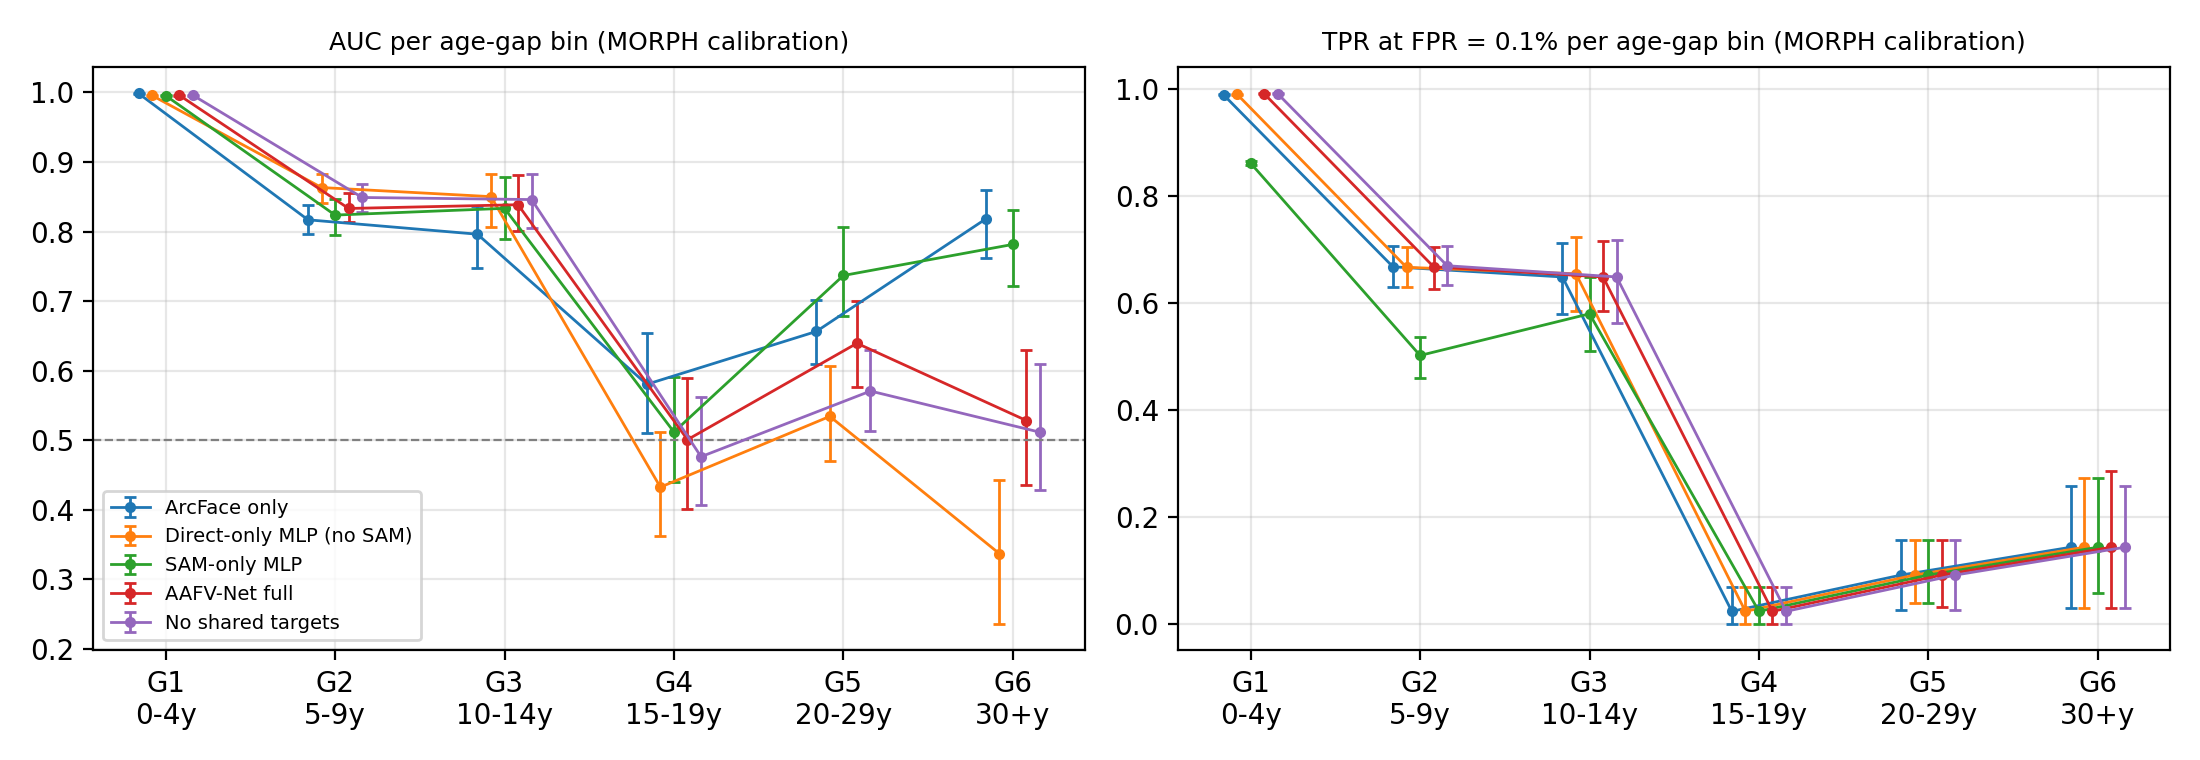
\includegraphics[width=\linewidth]{figures/fig_gap_ranking.png}
\caption{Ranking quality per age-gap bin on the MORPH calibration split for five variants (95\% intervals). Left: AUC. Right: TAR at FPR $=10^{-3}$. Bins of 15 years and more are analysed in Section~\ref{sec:labels}.}
\label{fig:gap}
\end{figure}

\subsection{Generated faces add no evidence at matched operating points}
\label{sec:generated}
Table~\ref{tab:matched} compares, on identical pairs, ArcFace on the original pair, ArcFace on the generated pairs (the score entering the SAM branch), the fused AAFV-Net score, and a person-cross-fitted logistic regression on the two ArcFace scores. Against random impostors the generated-pair score is significantly weaker than the original-pair score at 0--4 years ($\Delta$TAR $=-0.076$) and 5--9 years ($-0.072$), and combining the two changes TAR by exactly zero in every bin. At 5--9 years the generated-pair score has a nominally higher AUC ($+0.043$, 95\% CI $[0.000, 0.106]$), but this does not survive at the low false-match rates where decisions are made, and the combined score's AUC is not higher ($-0.026$, $[-0.065, +0.003]$). The fused score is slightly below ArcFace at 0--4 years ($-0.002$, $[-0.004,-0.001]$).

\begin{table}[t]
\centering
\caption{Per-pair comparison at matched false-match rate (FMR $=10^{-3}$) on the MORPH calibration split. $\Delta$ is the difference in TAR from ArcFace on the original pair, with a 95\% paired two-way person-cluster bootstrap interval (300 replicates). For gaps of 15 years and more every score has the same TAR against random impostors (15--19 y: 0.023 (n=44); 20--29 y: 0.091 (n=77); 30+ y: 0.143 (n=35)); those bins are analysed in Section~\ref{sec:labels}.}
\label{tab:matched}
\footnotesize
\setlength{\tabcolsep}{3pt}
\fittab{\begin{tabular}{@{}llccc@{}}
\toprule
Gap, y ($n$ gen.) & Score & TAR & $\Delta$TAR [95\% CI] & AUC \\
\midrule
\multicolumn{5}{@{}l}{\emph{Random impostors}} \\
0--4 (22914) & ArcFace (original pair) & 0.996 & -- & 0.999 \\
 & ArcFace (generated pair) & 0.920 & -0.076 [-0.112, -0.051] & 0.999 \\
 & AAFV-Net fused & 0.994 & -0.002 [-0.004, -0.001] & 0.996 \\
 & LogReg: original $+$ generated & 0.996 & +0.000 [+0.000, +0.000] & 0.999 \\
\addlinespace[1pt]
5--9 (594) & ArcFace (original pair) & 0.682 & -- & 0.840 \\
 & ArcFace (generated pair) & 0.609 & -0.072 [-0.111, -0.032] & 0.883 \\
 & AAFV-Net fused & 0.668 & -0.013 [-0.024, +0.000] & 0.807 \\
 & LogReg: original $+$ generated & 0.682 & +0.000 [+0.000, +0.000] & 0.814 \\
\addlinespace[1pt]
10--14 (174) & ArcFace (original pair) & 0.655 & -- & 0.813 \\
 & ArcFace (generated pair) & 0.644 & -0.011 [-0.045, +0.000] & 0.766 \\
 & AAFV-Net fused & 0.649 & -0.006 [-0.024, +0.000] & 0.821 \\
 & LogReg: original $+$ generated & 0.655 & +0.000 [+0.000, +0.000] & 0.806 \\
\addlinespace[1pt]
\multicolumn{5}{@{}l}{\emph{ArcFace-mined look-alikes}} \\
0--4 (22914) & ArcFace (original pair) & 0.985 & -- & 0.996 \\
 & ArcFace (generated pair) & 0.391 & -0.594 [-0.689, -0.513] & 0.974 \\
 & AAFV-Net fused & 0.988 & +0.003 [+0.001, +0.006] & 0.998 \\
 & LogReg: original $+$ generated & 0.981 & -0.004 [-0.006, -0.001] & 0.996 \\
\addlinespace[1pt]
5--9 (594) & ArcFace (original pair) & 0.653 & -- & 0.682 \\
 & ArcFace (generated pair) & 0.293 & -0.360 [-0.559, -0.117] & 0.683 \\
 & AAFV-Net fused & 0.653 & +0.000 [-0.012, +0.014] & 0.988 \\
 & LogReg: original $+$ generated & 0.653 & +0.000 [-0.012, +0.013] & 0.683 \\
\addlinespace[1pt]
10--14 (174) & ArcFace (original pair) & 0.649 & -- & 0.655 \\
 & ArcFace (generated pair) & 0.397 & -0.253 [-0.479, -0.059] & 0.647 \\
 & AAFV-Net fused & 0.649 & +0.000 [+0.000, +0.355] & 0.992 \\
 & LogReg: original $+$ generated & 0.649 & +0.000 [+0.000, +0.000] & 0.655 \\
\addlinespace[1pt]
\bottomrule
\end{tabular}}
\end{table}


\begin{figure}[t]
\centering
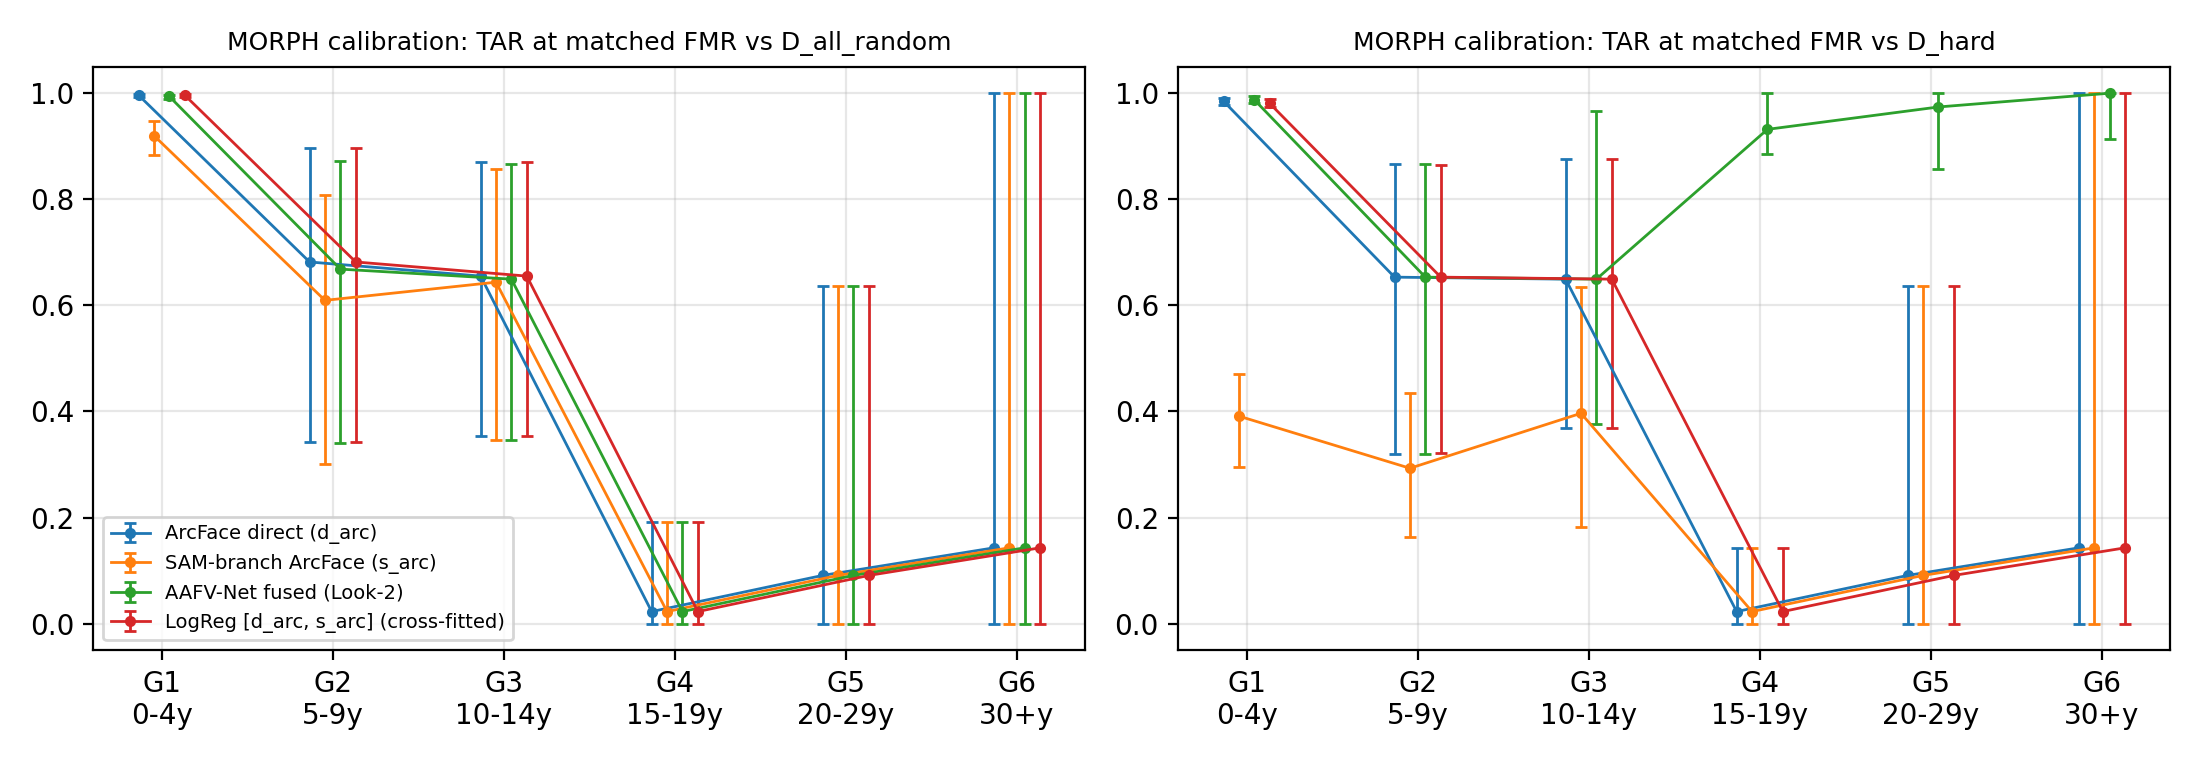
\includegraphics[width=\linewidth]{figures/fig_matched_fmr.png}
\caption{TAR at matched FMR per gap bin on the MORPH calibration split for the four scores of Table~\ref{tab:matched}, against random impostors (left) and ArcFace-mined look-alikes (right); 95\% person-cluster bootstrap intervals.}
\label{fig:matched}
\end{figure}

Against ArcFace-mined look-alikes the fused score gains $+0.003$ at 0--4 years, while the generated-pair score alone is much weaker (TAR 0.391 versus 0.985) and the two-score combination is not better than ArcFace. The strong look-alike rejection of Table~\ref{tab:test} therefore does not come from the generated evidence. It is shared by a direct-only variant without any SAM input (Table~\ref{tab:decision}: TPR 0.971 versus 0.973) and is consistent with half of the training negatives having been mined in the same way, which places $\mathcal{D}_\mathrm{hard}$ in the training distribution. The very large gains at 15 years and more in Fig.~\ref{fig:matched} (right) arise because the fused network scores mined look-alikes below even the mislabelled ``genuine'' pairs described in Section~\ref{sec:labels}; they are not evidence of long-gap capability.

\subsection{What the fusion network learned}
\label{sec:probe}
Table~\ref{tab:probe} inspects the frozen network. The original-pair head places almost all of its weight on ArcFace; EfficientNet, VGG-Face, LPIPS and SSIM receive weights an order of magnitude smaller. Moving the original-pair logit across its plausible range changes the fused logit about six times more than moving the generated-pair logit, and the response to the generated-pair logit and to $R_\mathrm{sam}$ is no larger than that of variants trained with those inputs held constant, whose response is arbitrary. Gap and quality are used modestly. The fused score is, in effect, a monotone transform of ArcFace with small context-dependent offsets, which explains Sections~\ref{sec:decision} and~\ref{sec:generated}.

\begin{table}[t]
\centering
\caption{What the frozen fusion network uses. Top: weights of the two linear branch heads on the five z-scored similarities (mean of 3 seeds). Bottom: change of the fused logit when one input moves across a plausible range (branch logits: bias $\pm 3\|w\|$; gap 5$\to$25 y; quality 0.3$\to$0.9; $R_\mathrm{sam}$ 0.2$\to$0.9). Untrained controls are variants trained with that input held constant, whose response is arbitrary.}
\label{tab:probe}
\footnotesize
\setlength{\tabcolsep}{4pt}
\fittab{\begin{tabular}{@{}lccccc@{}}
\toprule
Head & ArcFace & EfficientNet & VGG-Face & LPIPS & SSIM \\
\midrule
Original pair & -0.255 & +0.005 & -0.011 & +0.016 & -0.010 \\
Generated pairs & -0.101 & +0.149 & -0.057 & -0.004 & +0.023 \\
\bottomrule
\end{tabular}}

\vspace{4pt}
\fittab{\begin{tabular}{@{}lcc@{}}
\toprule
Input & Swing (full model) & Untrained control \\
\midrule
Original-pair branch logit & 25.1 & -- \\
Generated-pair branch logit & 4.1 & 4.4 (direct-only) \\
Synthesis reliability $R_\mathrm{sam}$ & 0.40 & 0.51 (no context) \\
Age gap & 0.90 & 0.23 (no context) \\
Image quality & 0.87 & 0.26 (no context) \\
\bottomrule
\end{tabular}}
\end{table}


\subsection{Integrity of the calibration procedure}
\label{sec:integrity}
The calibration code supported two post-hoc steps after inspecting a contact sheet of the highest-scoring calibration impostors: relabelling pairs and quarantining additional persons. The run logs show that the draft calibration of the original (five-network) model reached $T_\mathrm{acc}=1.0129$ at $\rho=0.20$, admitting nobody; the highest-scoring impostors were two pairs of persons with fused probabilities of 0.996 and 0.961. Of the 858 quarantined persons, 854 are explained by the automatic duplicate rule; the remaining four are exactly these two pairs. Restoring their 932 pairs (16 genuine, 4 person-disjoint random, 112 mined, 800 repeated random) raises $T_\mathrm{acc}$ above 1 and reduces genuine acceptance to 0\% for every value of $\rho$ (Table~\ref{tab:reconstruction}, bottom). Every acceptance rate reported for the system---73.26\% on calibration, 79.74\% and 70.07\% on the two test looks---depends on this removal. The images (Fig.~\ref{fig:morph}b shows other top-scoring pairs) would be needed to decide whether the four are duplicate records of two people or genuine look-alikes; in either case the step was taken after the scores were seen and must be reported.

The zero-failure bounds reported in earlier drafts are arithmetically correct (Table~\ref{tab:stats}), but they describe two different statements---a calibration-side certificate and a held-out audit, each with or without a multiplicity correction---and every method in Table~\ref{tab:decision}, including plain ArcFace, attains the same values, because all of them observe no random-impostor false accept. The calibration certificate further assumes that the scorer was fixed independently of the calibration impostors; the split was used to develop guards, variants and the floor $\rho$, and identities were removed after their scores were seen. We therefore do not regard these bounds as evidence about the method. They show that random-impostor risk is small at the $10^{-3}$ scale for every method considered; certifying $10^{-4}$ with zero observed errors would need about 30,000 independent impostor comparisons.

\begin{table}[t]
\centering
\caption{The zero-failure upper bounds $\varepsilon = 1-\delta^{1/n}$ on random-impostor FAR that appeared in earlier versions, recomputed. All are arithmetically correct; they describe two different statements (a calibration-side certificate and a held-out audit), and every method in Table~\ref{tab:decision} attains the same values.}
\label{tab:stats}
\footnotesize
\fittab{\begin{tabular}{@{}lccc@{}}
\toprule
Statement & $n$ & $\delta$ & $\varepsilon$ (\%) \\
\midrule
Calibration certificate & 1{,}170 & 0.05 & 0.256 \\
Calibration certificate, union over 3 values of $\rho$ & 1{,}170 & $0.05/3$ & 0.349 \\
Held-out audit, one look & 1{,}149 & 0.05 & 0.260 \\
Held-out audit, Bonferroni over 2 looks & 1{,}149 & 0.025 & 0.321 \\
\bottomrule
\end{tabular}}
\end{table}


\subsection{MORPH long-gap labels}
\label{sec:labels}
Every method reaches chance-level AUC at 15--19 years (Fig.~\ref{fig:gap}), which is implausible for modern recognizers on true adult pairs. Table~\ref{tab:labels} shows why. MORPH file names encode the subject's sex; within calibration ``same-person'' pairs the two names record different sexes in 0.0\% of pairs at 0--4 years but in 18--29\% at 15 years and more. Pairs whose file identifiers differ (a consequence of merging records with truncated or suffix-sharing identifiers into one person) are impostor-like far more often than pairs with matching identifiers at 5--14 years (58--80\% versus 5--8\%). On the test split, an independently trained Siamese ViT and the fused system find the same genuine pairs impostor-like (97\% at 15--19 years for both). The merge was correct for most short-gap pairs, which is why the problem went unnoticed; at long gaps it links different people, whose arbitrary age differences then appear as long gaps. Fig.~\ref{fig:morph}a shows examples from the pipeline's own audit sheet, including a pair recorded as one person whose two photographs differ visibly in sex and apparent ethnicity. As processed, MORPH contains essentially no valid long-gap genuine pairs, and the long-gap ``collapse'' reported for this system describes label errors rather than aging.

\begin{table*}[t]
\centering
\caption{Integrity of MORPH ``same-person'' pairs as processed by the pipeline. Sex mismatch: the sex letters encoded in the two file names differ. Impostor-like: the pair scores below the 99th percentile of random impostors in the same gap bin. Calibration columns use the direct ArcFace score; test columns are a post-hoc reading of logged outputs of the fused system (Look~1) and of an independently trained Siamese ViT.}
\label{tab:labels}
\footnotesize
\fittab{\begin{tabular}{@{}lccccccc@{}}
\toprule
 & \multicolumn{5}{c}{Calibration split} & \multicolumn{2}{c}{Test split (post hoc)} \\
\cmidrule(lr){2-6}\cmidrule(l){7-8}
Gap (y) & $n$ & Sex mismatch (\%) & File ids differ (\%) & Impostor-like (\%) & Impostor-like: ids differ / same (\%) & $n$ & Impostor-like: fused / ViT (\%) \\
\midrule
0--4 & 22,914 & 0.0 & 27.5 & 0.2 & 0.8 / 0.0 & 23631 & 0.4 / 4.3 \\
5--9 & 594 & 1.9 & 49.7 & 31.5 & 58.3 / 5.0 & 266 & 13.9 / 20.3 \\
10--14 & 174 & 2.9 & 36.8 & 34.5 & 79.7 / 8.2 & 184 & 23.9 / 23.9 \\
15--19 & 44 & 20.5 & 79.5 & 97.7 & 97.1 / 100.0 & 75 & 97.3 / 97.3 \\
20--29 & 77 & 18.2 & 77.9 & 90.9 & 96.7 / 70.6 & 137 & 94.9 / 97.8 \\
30+ & 35 & 28.6 & 65.7 & 85.7 & 91.3 / 75.0 & 12 & 0.0 / 0.0 \\
\bottomrule
\end{tabular}}
\end{table*}


\begin{figure}[t]
\centering
\includegraphics[width=\linewidth]{figures/faces_morph_audit.png}
\caption{Examples from the calibration audit sheets written by the pipeline (Look-1 model). (a) The lowest-scoring ``same-person'' pairs: the left pair is recorded as one person with a 12-year gap; the others illustrate genuinely hard captures (injury, expression). (b) The highest-scoring ``different-person'' pairs, several of which may be duplicate records of one person. Fused probability, gap and pair identifier are printed above each pair.}
\label{fig:morph}
\end{figure}

\subsection{How the generator changes faces}
Fig.~\ref{fig:samsheet} shows SAM outputs for two persons at three target ages, and Fig.~\ref{fig:change} where the generator changes the image. The largest changes are concentrated on the irises and eyebrows---the periocular region on which recognizers rely---together with regenerated background and clothing; the younger outputs lighten the eyes of both persons, and a distinctive joined eyebrow is thinned and split. Table~\ref{tab:sam} and Fig.~\ref{fig:sam} summarise all 379,930 SAM outputs. Similarity to the source falls from a median of 0.51 for shifts under 5 years to 0.35 for aging by 30 years or more, when 23\% of outputs fall below 0.30; aging degrades identity more than rejuvenation at large shifts, and age accuracy worsens from about 2 to about 5 years. These values come from the recognizer inside the pipeline, fed resized crops, so they describe the generator only relative to that recognizer; even a shift of a few years reduces the similarity to about 0.5, indicating that the generator rewrites the face substantially at every target age.

\begin{figure*}[t]
\centering
\includegraphics[width=0.92\textwidth]{figures/faces_sam_sheet.png}
\caption{SAM age progression for two persons. In each row, tiles 1, 3 and 5 are the original photograph and tiles 2, 4 and 6 are SAM outputs at a younger, a similar and an older target age.}
\label{fig:samsheet}
\end{figure*}

\begin{figure*}[t]
\centering
\includegraphics[width=0.92\textwidth]{figures/faces_sam_change_maps.png}
\caption{Where the generator edits the face. Each panel shows original $|$ SAM output $|$ per-pixel change (brighter = larger change), after aligning the output to the original. Changes concentrate on the irises and eyebrows; background and clothing are regenerated.}
\label{fig:change}
\end{figure*}

\begin{table}[t]
\centering
\caption{Identity similarity of SAM-generated faces to their source image (ArcFace cosine) and age accuracy, by direction and size of the age shift. ArcFace is the recognizer used inside AAFV-Net and received resized FFHQ crops, so these values are descriptive, not an independent identity test.}
\label{tab:sam}
\footnotesize
\setlength{\tabcolsep}{3pt}
\fittab{\begin{tabular}{@{}lcrcccc@{}}
\toprule
Direction & $|$shift$|$ (y) & $n$ & Median cos & 10th pct & $<0.30$ (\%) & Age error (y) \\
\midrule
older & 0--4 & 46,930 & 0.508 & 0.413 & 0.3 & 2.2 \\
older & 5--14 & 80,657 & 0.485 & 0.387 & 0.8 & 2.9 \\
older & 15--29 & 64,935 & 0.426 & 0.324 & 5.7 & 3.8 \\
older & 30+ & 12,613 & 0.352 & 0.261 & 23.1 & 4.8 \\
younger & 0--4 & 47,789 & 0.513 & 0.417 & 0.3 & 2.4 \\
younger & 5--14 & 77,512 & 0.500 & 0.402 & 0.6 & 3.2 \\
younger & 15--29 & 41,444 & 0.460 & 0.359 & 2.3 & 3.8 \\
younger & 30+ & 8,050 & 0.395 & 0.292 & 11.9 & 4.0 \\
\bottomrule
\end{tabular}}
\end{table}


\begin{figure}[t]
\centering
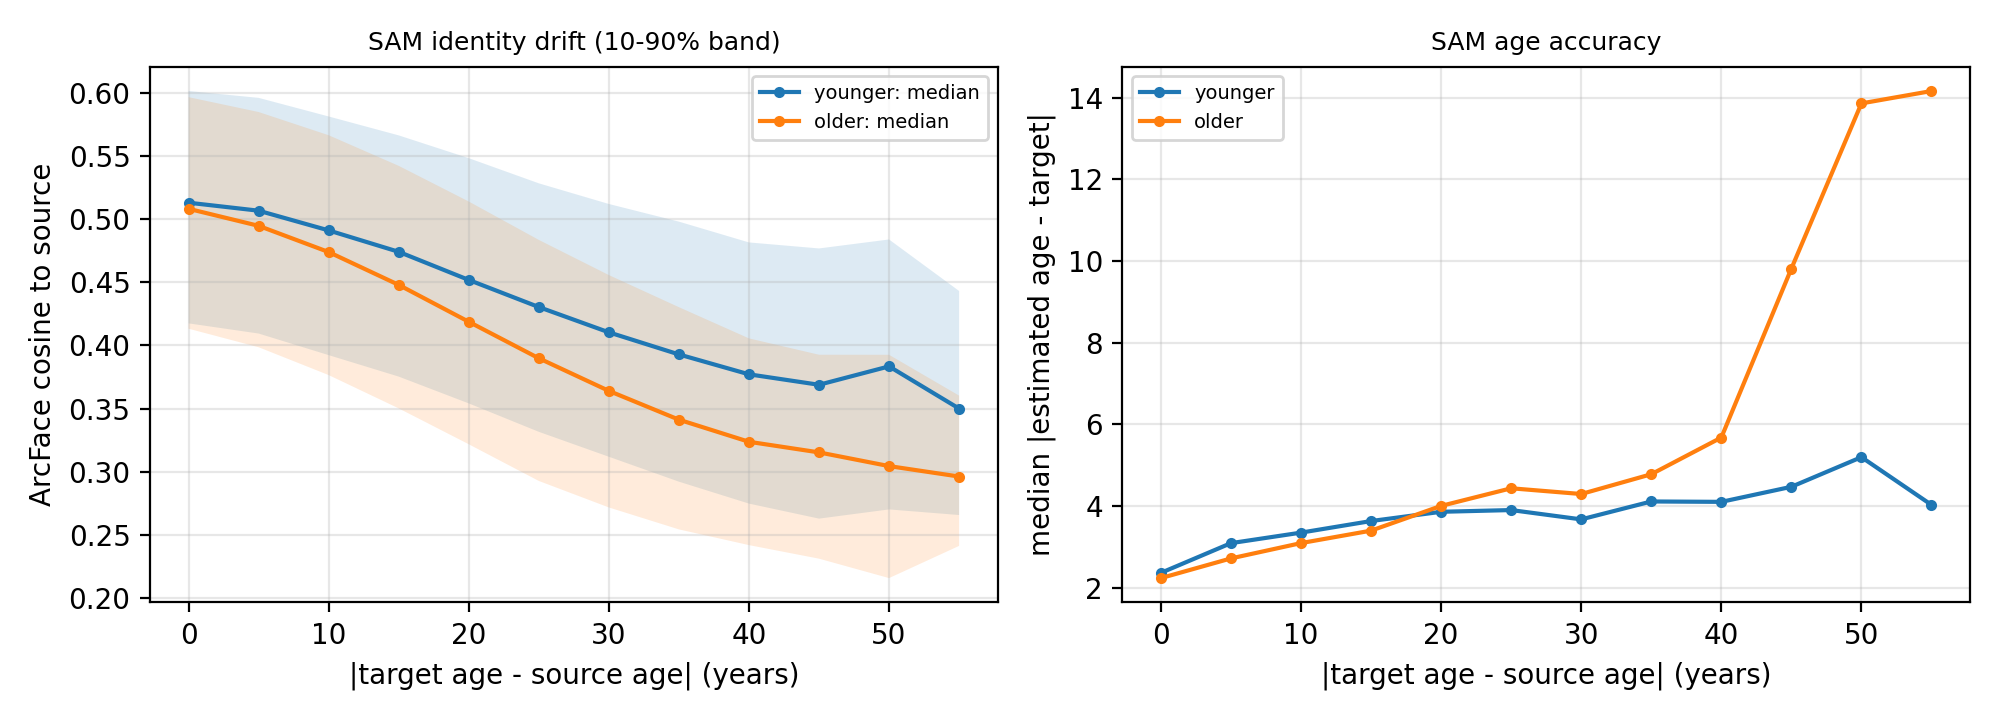
\includegraphics[width=\linewidth]{figures/fig_sam_drift.png}
\caption{All SAM outputs: ArcFace similarity to the source (median, 10--90\% band) and median age error, by size of the age shift and direction.}
\label{fig:sam}
\end{figure}

\subsection{External failures}
Fig.~\ref{fig:fgnet} shows the four FG-NET false accepts. All involve infants or toddlers photographed in poor, colour-cast scans, and all were accepted with fused probabilities of 0.966--1.000, although the persons are different by the dataset's labels. Guarded ArcFace made no false accept on the same impostor pairs, so these errors arise in the fused system; the recovered data contain no per-pair FG-NET scores, so the contribution of the synthetic branch to them cannot be isolated.

\begin{figure}[t]
\centering
\includegraphics[width=0.62\linewidth]{figures/faces_fgnet_false_accepts.png}
\caption{The four FG-NET false accepts (all ages, 20,000 impostor pairs), with image identifiers (person and age) and fused probabilities. All involve children aged 0--4.}
\label{fig:fgnet}
\end{figure}

\section{What Could Be Done}
\label{sec:future}
The audit leaves one question open: whether generated faces carry identity evidence at \emph{genuine} long gaps, under recognizers that are not part of the pipeline. MORPH cannot answer it, and AAFV-Net's design---test-time synthesis, hand-made reliability, guards around a fused score that reduces to ArcFace---cannot exploit it if the answer is yes. We therefore propose a different architecture and a test that must precede it. Nothing in this section has been run.

\subsection{Proposed architecture: reliability-weighted age transport}
Fig.~\ref{fig:proposed} shows the design. A frozen recognizer $f$ (AdaFace~\cite{kim2022adaface}, trained on a dataset that has not been withdrawn) embeds each face. A small transport head maps an embedding from its source age to a target age, $T_\theta(e,a,t)=\mathrm{normalize}(e+g_\theta[e,\gamma(a),\gamma(t)])$ with an age encoding $\gamma$, and predicts a von~Mises--Fisher concentration $\kappa_\theta(e,a,t)$. It is trained on real longitudinal pairs and on synthetic targets $f(G(I,t))$, each weighted by a learned reliability $w_\psi(\phi)$ computed from features of an \emph{independent} recognizer $h\ne f$, using learned loss attenuation~\cite{kendall2017uncertainty}:
\begin{multline}
\mathcal L=\mathcal L_\mathrm{real}+\eta\,\mathcal L_\mathrm{imp}\\
+\beta\sum_s\big[w_\psi(\phi_s)\,\ell_s-\lambda\log w_\psi(\phi_s)\big],
\end{multline}
where $\ell_s=\ell\big(T_\theta(e_s,a_s,t_s),f(G(I_s,t_s))\big)$ is the transport error on synthetic sample $s$.
At verification time no face is generated: the score is $S=\tfrac12[\kappa_{12}\,T_\theta(e_1,a_1,a_2)^\top e_2+\kappa_{21}\,e_1^\top T_\theta(e_2,a_2,a_1)]$, and the three-way rule~\eqref{eq:decision} is applied with thresholds fitted on a fresh calibration split, allowing a small number of calibration errors rather than none. The design differs from age-invariant training~\cite{wang2019dal,huang2021mtlface,wang2025ordcon} because the backbone is frozen; from quality-filtered synthetic fine-tuning~\cite{huang2022mtlfacetpami,banerjee2023aging} because reliability is a continuous, learned weight validated against an independent recognizer; and from AAFV-Net because synthesis is used only during training. Table~\ref{tab:plan} lists the ablations that would establish each component.

\begin{figure*}[t]
\centering
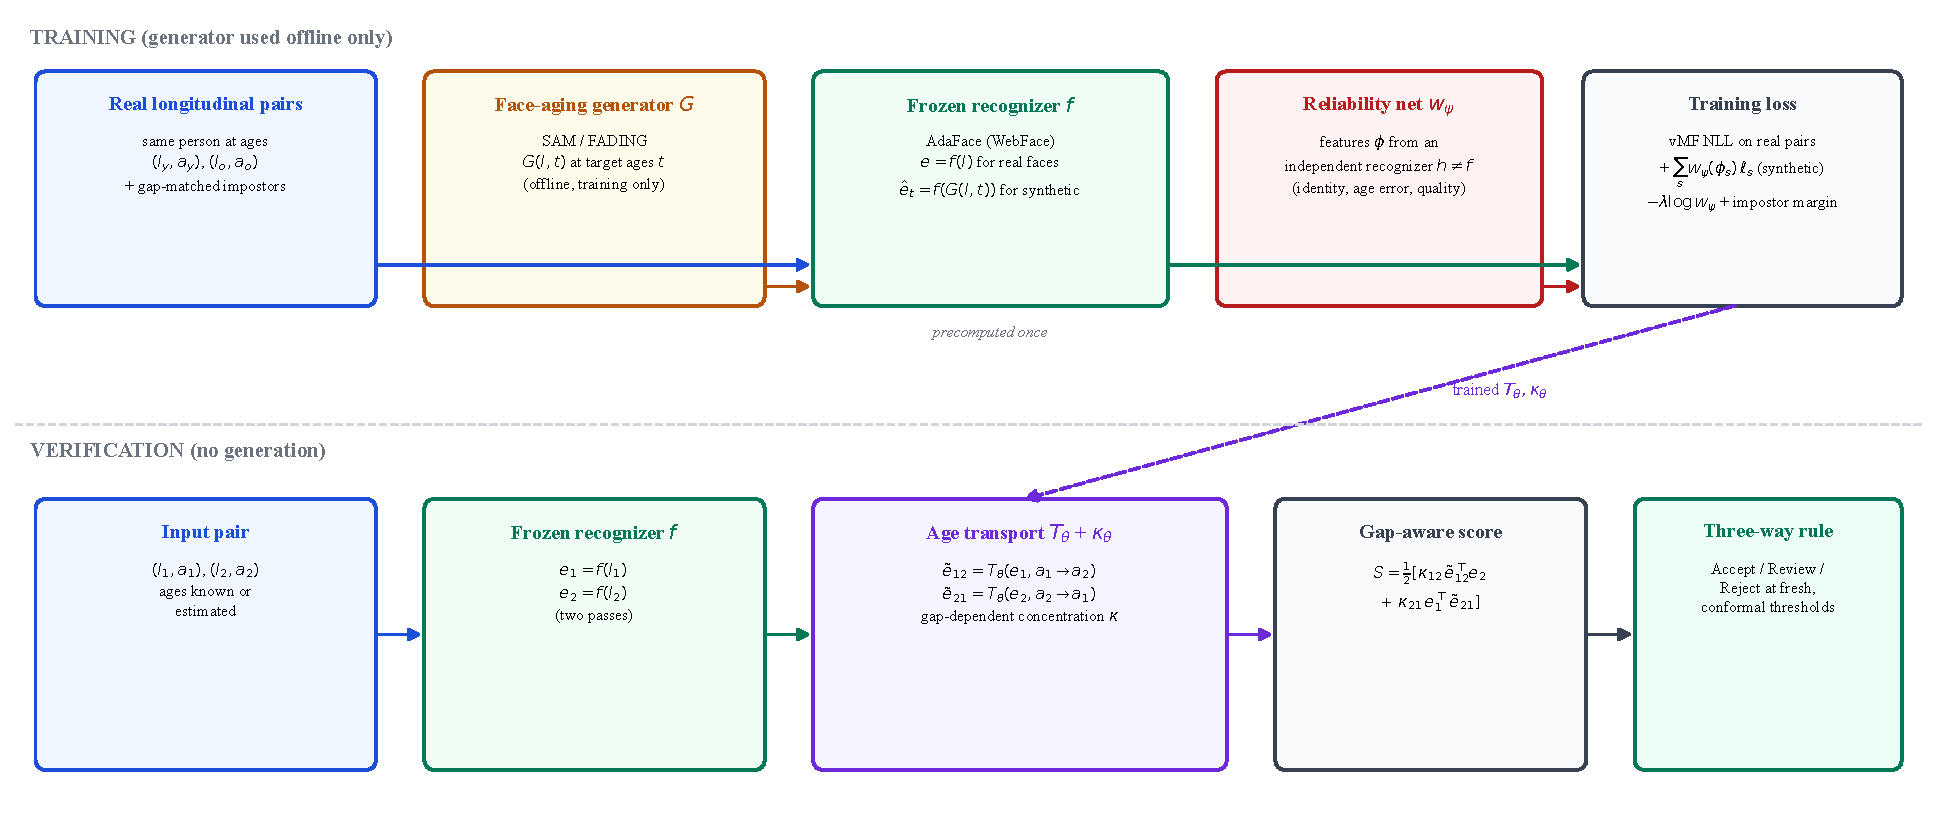
\includegraphics[width=\textwidth]{figures/fig_proposed_architecture.pdf}
\caption{Proposed reliability-weighted age-transport architecture (not evaluated). Top: training, with the generator used offline to produce synthetic targets weighted by a reliability network fed by an independent recognizer. Bottom: verification with two passes of a frozen recognizer, an age-transport head with gap-dependent concentration, and the three-way rule.}
\label{fig:proposed}
\end{figure*}

\begin{table}[t]
\centering
\caption{Planned ablation ladder for the proposed age-transport model (Fig.~\ref{fig:proposed}). Each row changes one component. \emph{No row has been run}; the last column states the outcome that would support the design, not a result.}
\label{tab:plan}
\footnotesize
\setlength{\tabcolsep}{3pt}
\fittab{\begin{tabular}{@{}clll@{}}
\toprule
\# & Variant & Isolates & Supports the design if \\
\midrule
1 & Recognizer cosine & -- & reference \\
2 & + gap/quality-conditioned calibration & context & small gain \\
3 & + transport head, real pairs only & transport & gain where real long gaps exist \\
4 & + synthetic targets, unweighted & synthetic data & mixed effect \\
5 & + synthetic, fixed hand-made weights & hand-made reliability & between rows 4 and 6 \\
6 & + synthetic, learned reliability & learned reliability & best long-gap TAR \\
7 & row 6 without $\kappa$ & uncertainty & worse risk--coverage \\
8 & generator or backbone swap & dependence & same ordering of rows \\
\bottomrule
\end{tabular}}
\end{table}


\subsection{A pre-registered test that must come first}
Before building the model, the following test decides whether generated faces carry identity evidence at all. It uses AgeDB~\cite{moschoglou2017agedb} and FG-NET~\cite{lanitis2002fgnet}; person-disjoint folds with all pairs formed within a fold; impostors formed by replacing the older image with a different person of matched age and sex, so that the younger image is progressed by the same generator call for genuine and impostor pairs; recognizers outside the pipeline (AdaFace~\cite{kim2022adaface} and MagFace~\cite{meng2021magface}, with standard five-point alignment); two generators (SAM~\cite{alaluf2021sam} and FADING~\cite{chen2023fading}); a person-cross-fitted combination of original and generated scores; and an age-only control in which each generated face is replaced by a different person's face generated at the same target age. The decision criterion is a gain in TAR at FMR $10^{-3}$ in the 15--29 or 30+ year adult bins whose Bonferroni-adjusted interval excludes zero, with no gain under the control. The full pre-registration and tested code accompany this paper. A negative outcome would mean that generated aging should not be used as verification evidence on these data; a positive one would justify the model of Fig.~\ref{fig:proposed}.

\subsection{Data for long gaps}
Long-gap evidence must come from datasets with valid long-gap identity labels. AgeDB contains about 29 images per person with ages from 1 to 101; FG-NET spans ages 0--69 but has only 82 persons; LAG~\cite{bianco2017lag} pairs young and adult photographs of about a thousand persons but has no age labels; CACD~\cite{chen2014cacd} spans only about a decade; CALFW~\cite{zheng2017calfw} estimates ages; and celebrity datasets may overlap recognizer pretraining. Any MORPH use requires the linkage audit of Section~\ref{sec:labels} first, and label-noise-tolerant training~\cite{deng2020subcenter} may help where errors cannot be removed.

\section{Discussion}
\textbf{What generalises.} Three lessons extend beyond this system. First, comparisons of selective verifiers must be made at matched false-match rates and matched review workload; a decision layer can create or hide large differences in automation between methods that discriminate identically. Second, synthetic evidence should be tested per pair against the recognizer it is meant to help, with a combination model fitted out of sample; aggregate system results cannot separate its contribution. Third, longitudinal datasets need linkage audits before long-gap claims: the errors here are concentrated exactly where the scientific claim lives.

\textbf{Threat model.} The random-impostor bounds concern zero-effort impostors of the same sex from the calibration population. They say nothing about look-alikes chosen by an adversary~\cite{hu2025neyman,paone2014twins}, about morphing or presentation attacks~\cite{scherhag2019morph,iso30107_3}, about synthetic forgeries~\cite{zhou2024openset}, or about attacks on stored templates~\cite{otroshi2024inversion}. Long-term face matching also raises privacy concerns~\cite{razeghi2026privacy}, and accuracy differs across demographic groups~\cite{klare2012demographics,grother2019frvt_part3,krishnapriya2020race,buolamwini2018gendershades}: on the first test look, guarded acceptance was 81.07\% for male and 71.93\% for female genuine pairs. Calibration of the probability itself is a further open issue~\cite{guo2017calibration,naeini2015ece,brier1950,xu2024asc}.

\section{Limitations}
All controlled comparisons use the MORPH calibration split, which was also used during the development of AAFV-Net; they are re-analyses of a fixed model, not new confirmatory evaluations. The identity measurements use the pipeline's own recognizer with non-standard alignment. The label analysis relies on file names and scores; a visual audit of a sample of long-gap pairs is needed to estimate the error rate precisely. Whether the four removed identities are duplicates is unresolved. FG-NET results could not be re-analysed. The test-split readings are post hoc. The proposed architecture and protocol are designs, not results.

\section{Conclusion}
AAFV-Net frames cross-age verification as a guarded three-way decision with synthetic age-progression evidence. Re-examined at matched operating points, its synthetic branch contributes no verification evidence beyond ArcFace on MORPH, its acceptance deficit is a property of its decision layer, its published operating point depends on a post-hoc calibration exclusion, and the long-gap MORPH pairs on which age-related conclusions would rest are largely mislabelled. The reject-option framing, the data hygiene and the insight that synthetic evidence must be trusted selectively remain useful. We propose an architecture that uses generated faces only as reliability-weighted training signal for a frozen recognizer, and a pre-registered test that must succeed before it is built.

\section*{Data and Code Availability}
MORPH and FG-NET are available from their providers under licence; no images are redistributed with the code. Analysis scripts, aggregate result tables, the hash manifest of the frozen models and the pre-registered protocol are available from the authors [repository to be confirmed].

\section*{Ethics Statement}
This study uses existing, licensed face datasets and creates no new data from human participants. [Institutional review status to be confirmed by the authors.] The face images shown are taken from these datasets for illustration and must be cleared under their licences before publication. MORPH consists of arrest photographs with a skewed demographic composition; results should not be generalised to other populations, and long-term face matching carries surveillance risks that deployments must address.

\section*{Use of AI Tools}
An AI assistant (Claude, Anthropic) was used to write and verify the analysis code, to check references against their sources, to generate figures and tables from logged results, and to draft this manuscript under the authors' direction. All reported numbers are produced by scripts and were checked against their sources. The authors are responsible for the content. [To be revised and confirmed by the authors before submission.]

\bibliographystyle{IEEEtran}
\bibliography{references}

\end{document}
